\documentclass[aip,jcp,reprint]{revtex4-1} 
\usepackage{graphicx}
\usepackage{enumitem}

\usepackage{mathtools}
\usepackage{graphicx}   
\usepackage{color}
\usepackage{ulem}
\usepackage{caption}
\usepackage{subcaption}

\usepackage{caption}
\usepackage[version-1-compatibility]{siunitx}

\usepackage{array}
\newcolumntype{C}[1]{>{\centering\arraybackslash}p{#1}} 
\captionsetup[figure]{labelfont=bf,
                    textfont=normalfont,
                    justification=RaggedRight}
\captionsetup[table]{labelfont=bf,
                    textfont=normalfont,
                    justification=RaggedRight}

\usepackage{booktabs}
\usepackage{multirow}
\newcommand{\head}[1]{\textnormal{\textbf{#1}}}
\newcommand{\normal}[1]{\multicolumn{1}{l}{#1}}

\usepackage{booktabs}
\newcommand{\ra}[1]{\renewcommand{\arraystretch}{#1}}




\begin{document}
\title{Optical pumping to a single hyperfine projection of the rovibrational ground-state of AlH$^+$ molecules}

	
	
	\author{Panpan Huang}
 \affiliation{Department of Physics and Astronomy, Northwestern University, Evanston, IL 60208, USA}

	\author{Schuyler Kain}
 \affiliation{Department of Physics and Astronomy, Northwestern University, Evanston, IL 60208, USA}

    \author{Antonio de Oliveira-Filho}
 \affiliation{Departamento de Química, Faculdade de Filosofia, Ciências e Letras de Ribeirão Preto, Universidade de São Paulo, Ribeirão Preto-SP 14040-901, Brazil}

 \author{Brian Odom*}
 \email{b-odom@northwestern.edu}
 \affiliation{Department of Physics and Astronomy, Northwestern University, Evanston, IL 60208, USA}
 
	\date{\today}

\begin{abstract}
In this work we propose an optical pumping scheme to cool trapped AlH$^+$ molecules to the stretched hyperfine state ($\lvert F=7/2, m_F=7/2\rangle$) of the rovibrational ground state ($\lvert X^2\Sigma^+, v=0, N=0\rangle$) using the combination of a linearly polarized and a circularly polarized broadband pulsed laser to cool down the rotational degree of freedom and drive the population to the stretched hyperfine state respectively. We also found that adding a laser coupling a specific transition between $v=1$ and $v=0$ in the  $ X^2\Sigma^+$ state can accelerate the cooling process. The hyperfine coupling constants of the $A^2\Pi$ state and the$X^2\Sigma^+$ state are also calculated since the lasers couple the transitions between the hyperfine states of $\lvert X^2\Sigma^+, v=0\rangle$ and $\lvert A^{2}\Pi, v=0\rangle$ in AlH$^+$ but only some hyperfine constants of the $X^{2}\Sigma^+$ have been measured or calculated. Applying the calculated hyperfine structures in the simulation of population dynamics solving rate equations, we show that under optimum conditions, the population in the stretched hyperfine state of the rovibrational gorund state can reach $63.2\, \%$ after 80 {\micro}s/276.2 ms and $95.4\, \%$ after 2.04 ms/1.058 s with/without the vibrational coupling laser on.
\end{abstract}


	\maketitle
	
\section{Introduction}
%applicaitons
Laser cooling the internal energies of molecular ion has become an intense research. It's essential in many applications including precision measurement[cite], quantum simulation[cite], quantum information processing[cite] and the study of state-dependent reaction in cold chemistry[cite]. In the measurement of the variation of the $m_p/m_e$, the near degenerate transitions of molecules can enhance the sensitivity coefficient. The rich internal degrees of freedom and the long range interaction offer possibilities of developing the quantum toolkit in both quantum simulation and quantum information processing. Preparation of molecules to a single quantum state is also required in some studies of the ultracold collision in cold chemistry. In addition to the preferable nature of molecule mentioned above, the long interrogation time provided by the ion trap allows us to do a better control and study a broader set of molecules.\par
% Others
There are some previous efforts on achieving a single populated quantum state of neutral molecules. Some groups perform the quantum state preparation in the process of synthesizing the molecules through photo-association of atoms followed by an stimulated Raman adiabatic transition[cite]. In their works, the constituted atoms of the molecules need to be trapped in the magneto-optical trap (MOT) before synthesizing, and the conversion efficiency is reported to be around 75 $\%$ and 84 $\%$.\par

Cooling of internal states and manipulating the population in certain hyperfine states of the molecular ion, HD$^+$ is also demonstrated[cite].The rotational cooling is obtained by optical pumping specific vibrational transitions and vibrational relaxations. Meanwhile, the blackbody radiation (BBR) induced transition redistributes the population from higher vibrational states into the lower vibrational states which can be coupled by the optical pumping lasers. In their experimental demonstration, the rovibrational ground state population can reach 75 $\%$ after few tens of second. The rotational cooling time scale is limited by the BBR redistribution rate ($\sim$ 1 s). Manipulation of the population among specific hyperfine states can be then performed by coupling individual hyperfine states in those involved rovibrational levels through optical excitation using a frequency-comb-based, continuous-wave laser, and achieving controlled transfer of population into a selected hyperfine state[cite]. The whole hyperfine population transfer process also takes few tens of seconds.\par

%Ours
It has been shown that the rotational cooling can be achieved using only a pulse-shaped femtosecond laser (PFL) on molecules with relatively large rotational constants and fairly diagonal Frank-Condon factors (FCFs)[cite]. In particular, for AlH$^+$, our group has demonstrated the rotational ground state population has increased from a few percent to about 95.4 $\%$ within a second\cite{lien2014broadband}. However, this method has limited by its nature of not being able to prepare the population to a single quantum state since the spin interaction generates hyperfine structure in each rovibrational manifold. For example, the rovibronic ground state of AlH$^+$ has one unpaired electron (spin $s_{e}=1/2$), and nuclei with nuclear spins $I_{1}=5/2$ and $I_{2}=1/2$ has 4 hyperfine states in zero magnetic field.\par
In this article, we proposed a method to further transfer the population to a single stretched hyperfine state of the rovibrational ground state in an efficient way. In Section II, we will explain our theory and method of rotational cooling, how we can accelerate the rotational cooling process, and further pump the system to the stretched hyperfine state. The simulation details will be shown in Section III. In Section IV, we will show our simulation results and discussion. The conclusion is arranged at Section V.\par

%past work
%the work in this paper
%https://journals.aps.org/prl/abstract/10.1103/PhysRevLett.108.183003

\section{Theory and Methods}
The time scale of the previous rotational cooling methods performed on HD$^+$ has been intrinsically limited to few tens of seconds due to the low BBR induced transition rate. 

Our group has demonstrated a rotational cooling method on AlH$^+$ molecules through optical pumping using a pulse-shaped linearly-polarized 360 nm from a frequency-doubled femtosecond laser (SpectraPhysics MaiTai) with a 80 MHz repetition rate, so each pulse has a comb-like frequency spectrum with frequency interval equal to the repetition rate. Its broadband nature allows us to pump many rotational transitions simultaneously, and the pulse-shaping technique allows us to select only the rotational cooling frequency components. We drive the selected P- and Q- branch of electronic transition of AlH$^+$ from $\lvert X^2\Sigma^+, v''=0\rangle$ to $\lvert A^{2}\Pi, v'=0\rangle$.\par
The cooling process has two parts. The first part contains cycles of the fast sequence of electronic excitation from $\lvert X^2\Sigma^+, v''=0\rangle$ to $\lvert A^{2}\Pi, v'=0\rangle$ each followed by a electronic relaxation. The electronic relaxation time is around 60 ns, thus the rotational state population can be driven into the two lowest rotational states, $\lvert v''=0, N''=0,1\rangle$, within only a few microseconds. However, since the selection rule for the transition driven by the linearly-polarized PFL between $\lvert X^2\Sigma^+\rangle$  and $\lvert A^2\Pi\rangle$ is $\Delta J=0, \pm 1$ and parity $+\longleftrightarrow -$. The population in $\lvert X^2\Sigma^+, v''=0, N''=1, -\rangle$ cannot be transferred to the rovibrational ground state, $\lvert X^2\Sigma^+, v''=0, N''=0, +\rangle$, through the fast sequence of absorbing and emitting a photon between electronic states because of parity. The population in $\lvert X^2\Sigma^+, v''=0, N''=1, -\rangle$ needs to go through a slower parity flipping process via the intermediate state, $\lvert X^2\Sigma^+, v''=1, N''=1, -\rangle$ to reach the rovibrational ground state as shown in Figure \ref{level_diagram_parity}, which is the relatively slow second part of the cooling process because the vibrational relaxation time from $\lvert X^2\Sigma^+, v=1\rangle$ to $\lvert X^2\Sigma^+, v=0\rangle$ is about 140 ms.

In our laboratory, AlH$^+$ ions are trapped in a linear Paul trap and initially sympathetically cooled to sub-Kelvin translational temperatures via their Coulomb interaction with Doppler-cooled co-trapped $\rm Ba^+$. To remove the dark states of barium ion during the Doppler cooling process, a magnetic field is always on around 2 G. After the translational cooling, the linearly polarized PFL which the polarization is perpendicular to the magnetic field is then turned on to rotationally cool the molecules into the rovibrational ground state.

To reduce the slowdown effect due to the vibrational decay, we propose to add a 6.8 {\micro}m continuous-wave laser which couples the transition between $\lvert X^2\Sigma^+, v''=1, N''=1, -\rangle$ and $\lvert X^2\Sigma^+, v''=0, N''=2, +\rangle$. By adding this laser, in the simulation, we show that the rotational cooling time scale can be shorten by about 3 orders of magnitude as shown in Figure \ref{RC_RCv10} and Table \ref{RC_RC_v10table}.

\begin{figure}[!h]
  \centering
  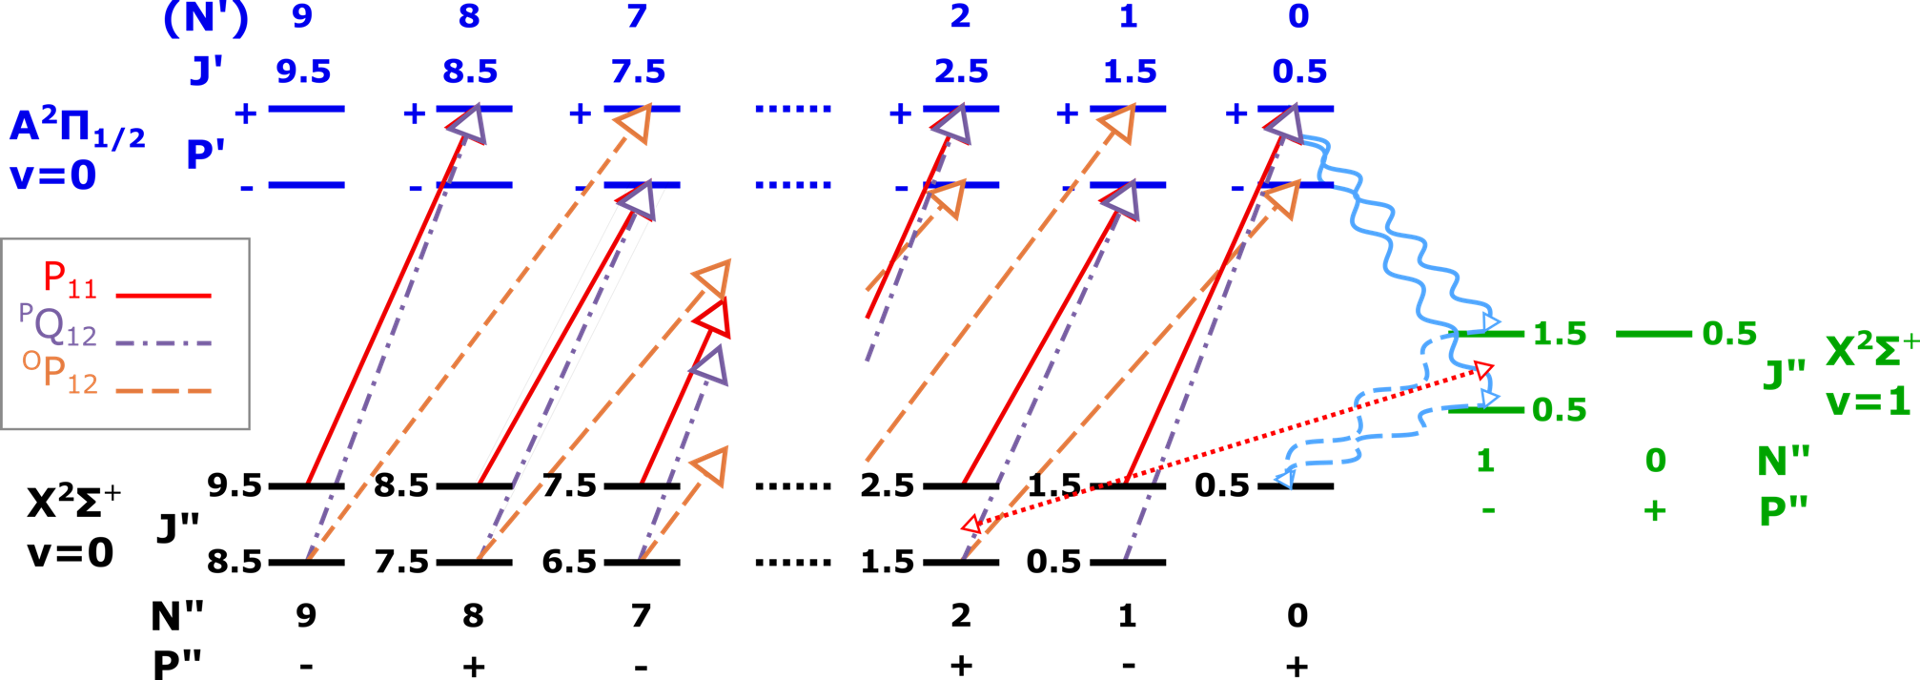
\includegraphics[width=8cm]{level_diagram_parity}
  \caption
  { level diagram parity.
}\label{level_diagram_parity}
\end{figure}

In order to further transfer our system to single quantum state, in addition to the linear polarized beam, we add a separated $\sigma^+$-polarized beam. We can then utilize the selection rule with the $\sigma^+$-polarized laser to optical pump the system to this stretched hyperfine state in which the spin and the rotational angular momentum are aligned with the quantization axis. The schematic plot of our setup is shown in Fig. \ref{schematic_setup}. When we apply the $\sigma^+$-polarized laser, the selection rule can be expressed as following:
\begin{align*}
\Delta F=0, \pm 1 \\
\Delta m_F=1
\end{align*}

\begin{figure}[!h]
  \centering
  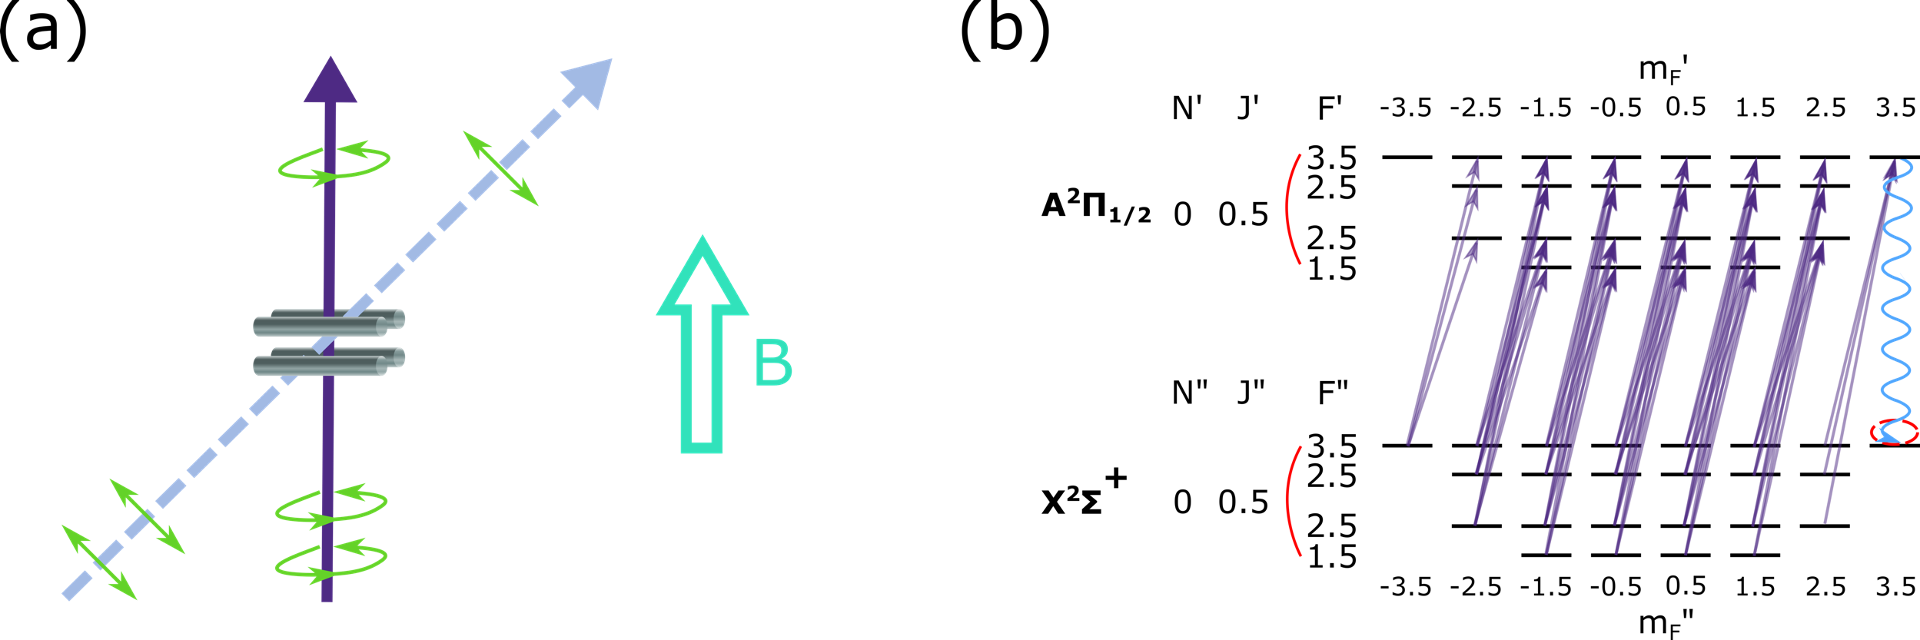
\includegraphics[width=8cm]{schematic_setup}
  \caption
  { schematic setup.
}\label{schematic_setup}
\end{figure}

where $F$ is the total angular momentum and $m_F$ is the projection quantum number. As can be seen in {Fig}, if we can park the $\sigma^+$-polarized laser to drive the Q(0) branch transitions from $\lvert X^2\Sigma^+, v''=0, N''=0\rangle$ to $\lvert A^2\Pi, v'=0, N'=0\rangle$, most of the population in the rovibrational ground state of $X^2 \Sigma+$ will go through the cycles of the sequence of absorbing a photon and spontaneous decaying and thus move toward the stretched hyperfine state. This selection rule will make the stretched hyperfine state a dark state which cannot absorb photon anymore because there is no higher $m_F$-state in the $\lvert A^2\Pi, v=0, N=0\rangle$; therefore the population will stay there. Our goal of single quantum state preparation is then achieved. 


\section{Simulation Detail} 
Our population dynamics is calculated through the following rate equation:
\begin{align}
\begin{aligned}
\frac{\partial\rho_i}{\partial t}=-\sum_{j\neq i}B_{i,j}(I_{BBR}+I_{laser})\rho_i - \sum_{j<i}A_{i,j}\rho_i \\
+\sum_{j\neq i}B_{j,i}(I_{BBR}+I_{laser})\rho_i + \sum_{j>i}A_{j,i}\rho_i 
\end{aligned}
\end{align}
where $\rho_i$ is the population fraction in state $i$. The initial population is assumed to be thermal populated at the room temperature 300K. $I_{BBR}$ and $I_{laser}$ are the energy densities of the black body radiation and laser. A and B are the Einstein coefficients.

\begin{align}
\begin{aligned}
A_{ul} = \frac{2\pi \widetilde{\nu}^2 q_e^2}{\epsilon_0 m_e c} \frac{g_l}{g_u} f_{lu}\\
B_{ul} = \frac{q_e^2}{4 \epsilon_0 m_e h c \widetilde{\nu}} \frac{g_l}{g_u} f_{lu} \\
B_{lu} = \frac{q_e^2}{4 \epsilon_0 m_e h c \widetilde{\nu}} f_{lu}\\
\end{aligned}
\end{align}

The Einstein A,B coefficients can be computed using equation (2) with the output transition energies and the transition oscillator strength from Western's Pgopher[reference]. In the calculation using Pgopher, the magnetic field is set to 10 G. To perform the calculation using Pgopher, we need the electronic state constants which is obtained from literature[reference?], the permanent dipole moments and the transition dipole moments which are calculated using Le Roy's LEVEL[reference?], the hyperfine constants and the nuclear quadrupole coupling constants of the $X^2\Sigma+$ and $A^2\Pi$ states are obtained using Dalton, and the Landé g-factors which are from[reference?].

The potential energy functions and the transition dipole moment function for the $X^2 \Sigma+$ and $A^2\Pi$ state were obtained from the literature[reference?] and have been used in LEVEL to calculate the permanent dipole moments and the transition dipole moments.

 In the calculation using Dalton, we choose the pcJ-1 basis set because pcJ family was developed for RMN/EPR spin-spin coupling constants and have tight functions, and thus should be well suited to describe the electron density near the nucleus. The density function theory (DFT) using the B3LYP density functional is applied with an pcJ-1 basis set to calculate the nuclear quadrupole coupling constants and hyperfine constants calculated in Dalton. The calculated results are shown in [Table XX].

At room temperature, 99 $\%$ of the AlH$^+$ population is in the lowest vibrational state v=0 in $X^2 \Sigma$, with the significant population distributed among the first 10 rotational levels, $J=0.5$-$9.5$, and less than $4\, \%$ in $J>9.5$.
The involved states in the rate equation simulation are  $J=0.5$-$9.5$ in $X^2\Sigma+ (v''=0,1)$ and $A^2\Pi (v'=0)$. We include $X^2\Sigma+ (v''=1)$ because in that way, we can simulate the parity flipping process via the intermediate state, $\lvert X^2\Sigma^+, v''=1, N''=1, -\rangle$. 
The bandwidth of the femtosecond laser is $7\, nm$ and set to be centered around 360 nm with the 80 MHz comb-like spectrum. We then apply an cut-off in the laser output spectrum to include the frequency range that drive selective P- and Q- branch rotational cooling transitions, namely the $P_{11}$, $P_{12}$ and the $^pQ_{12}$ branches for the linearly polarized PFL and set the cut-off frequency to include $Q_{12}(0)$ and the above rotational cooling transitions for the $\sigma^+$-polarized PFL. We assume the the final power from the frequency doubled femtosecond laser sent into the vacuum chamber has a power of 100 mW and been focused onto 200 {\micro}m radius spot for both the linearly polarized and the $\sigma^+$-polarized beam. 
The typical optical transition linewidth for AlH$^+$ between is 20 MHz, which is smaller than the comb interval of the $80\, MHz$ from the femtosecond laser. Therefore, it would be possible for the PFL to miss some of the transitions we desire to drive.
We solve this issue in the simulation by introducing the Doppler-broadened linewidth assuming the translational temperature of the AlH$^+$ ion cloud is $\sim 1\, K$, which ensures that the PFL can drive all the desired cooling transitions.  

In the experiment, one can increase the translational temperature of the AlH$^+$ ion cloud by directly exciting the secular motion of the AlH$^+$ with an oscillating electric field or pushing the entire ion cloud away from the geometric center of the Paul trap by applying a DC field to introduce excess micro motion, in which ions oscillate at the RF frequency with amplitude proportional to the applied DC field [reference?]. After internal cooling is finished, one can then turn off the translational temperture heating source, and the translationally hot molecular ions will again be sympathetically cooled by the laser-cooled Ba+.

\begin{figure*}[htbp!]
  \centering
  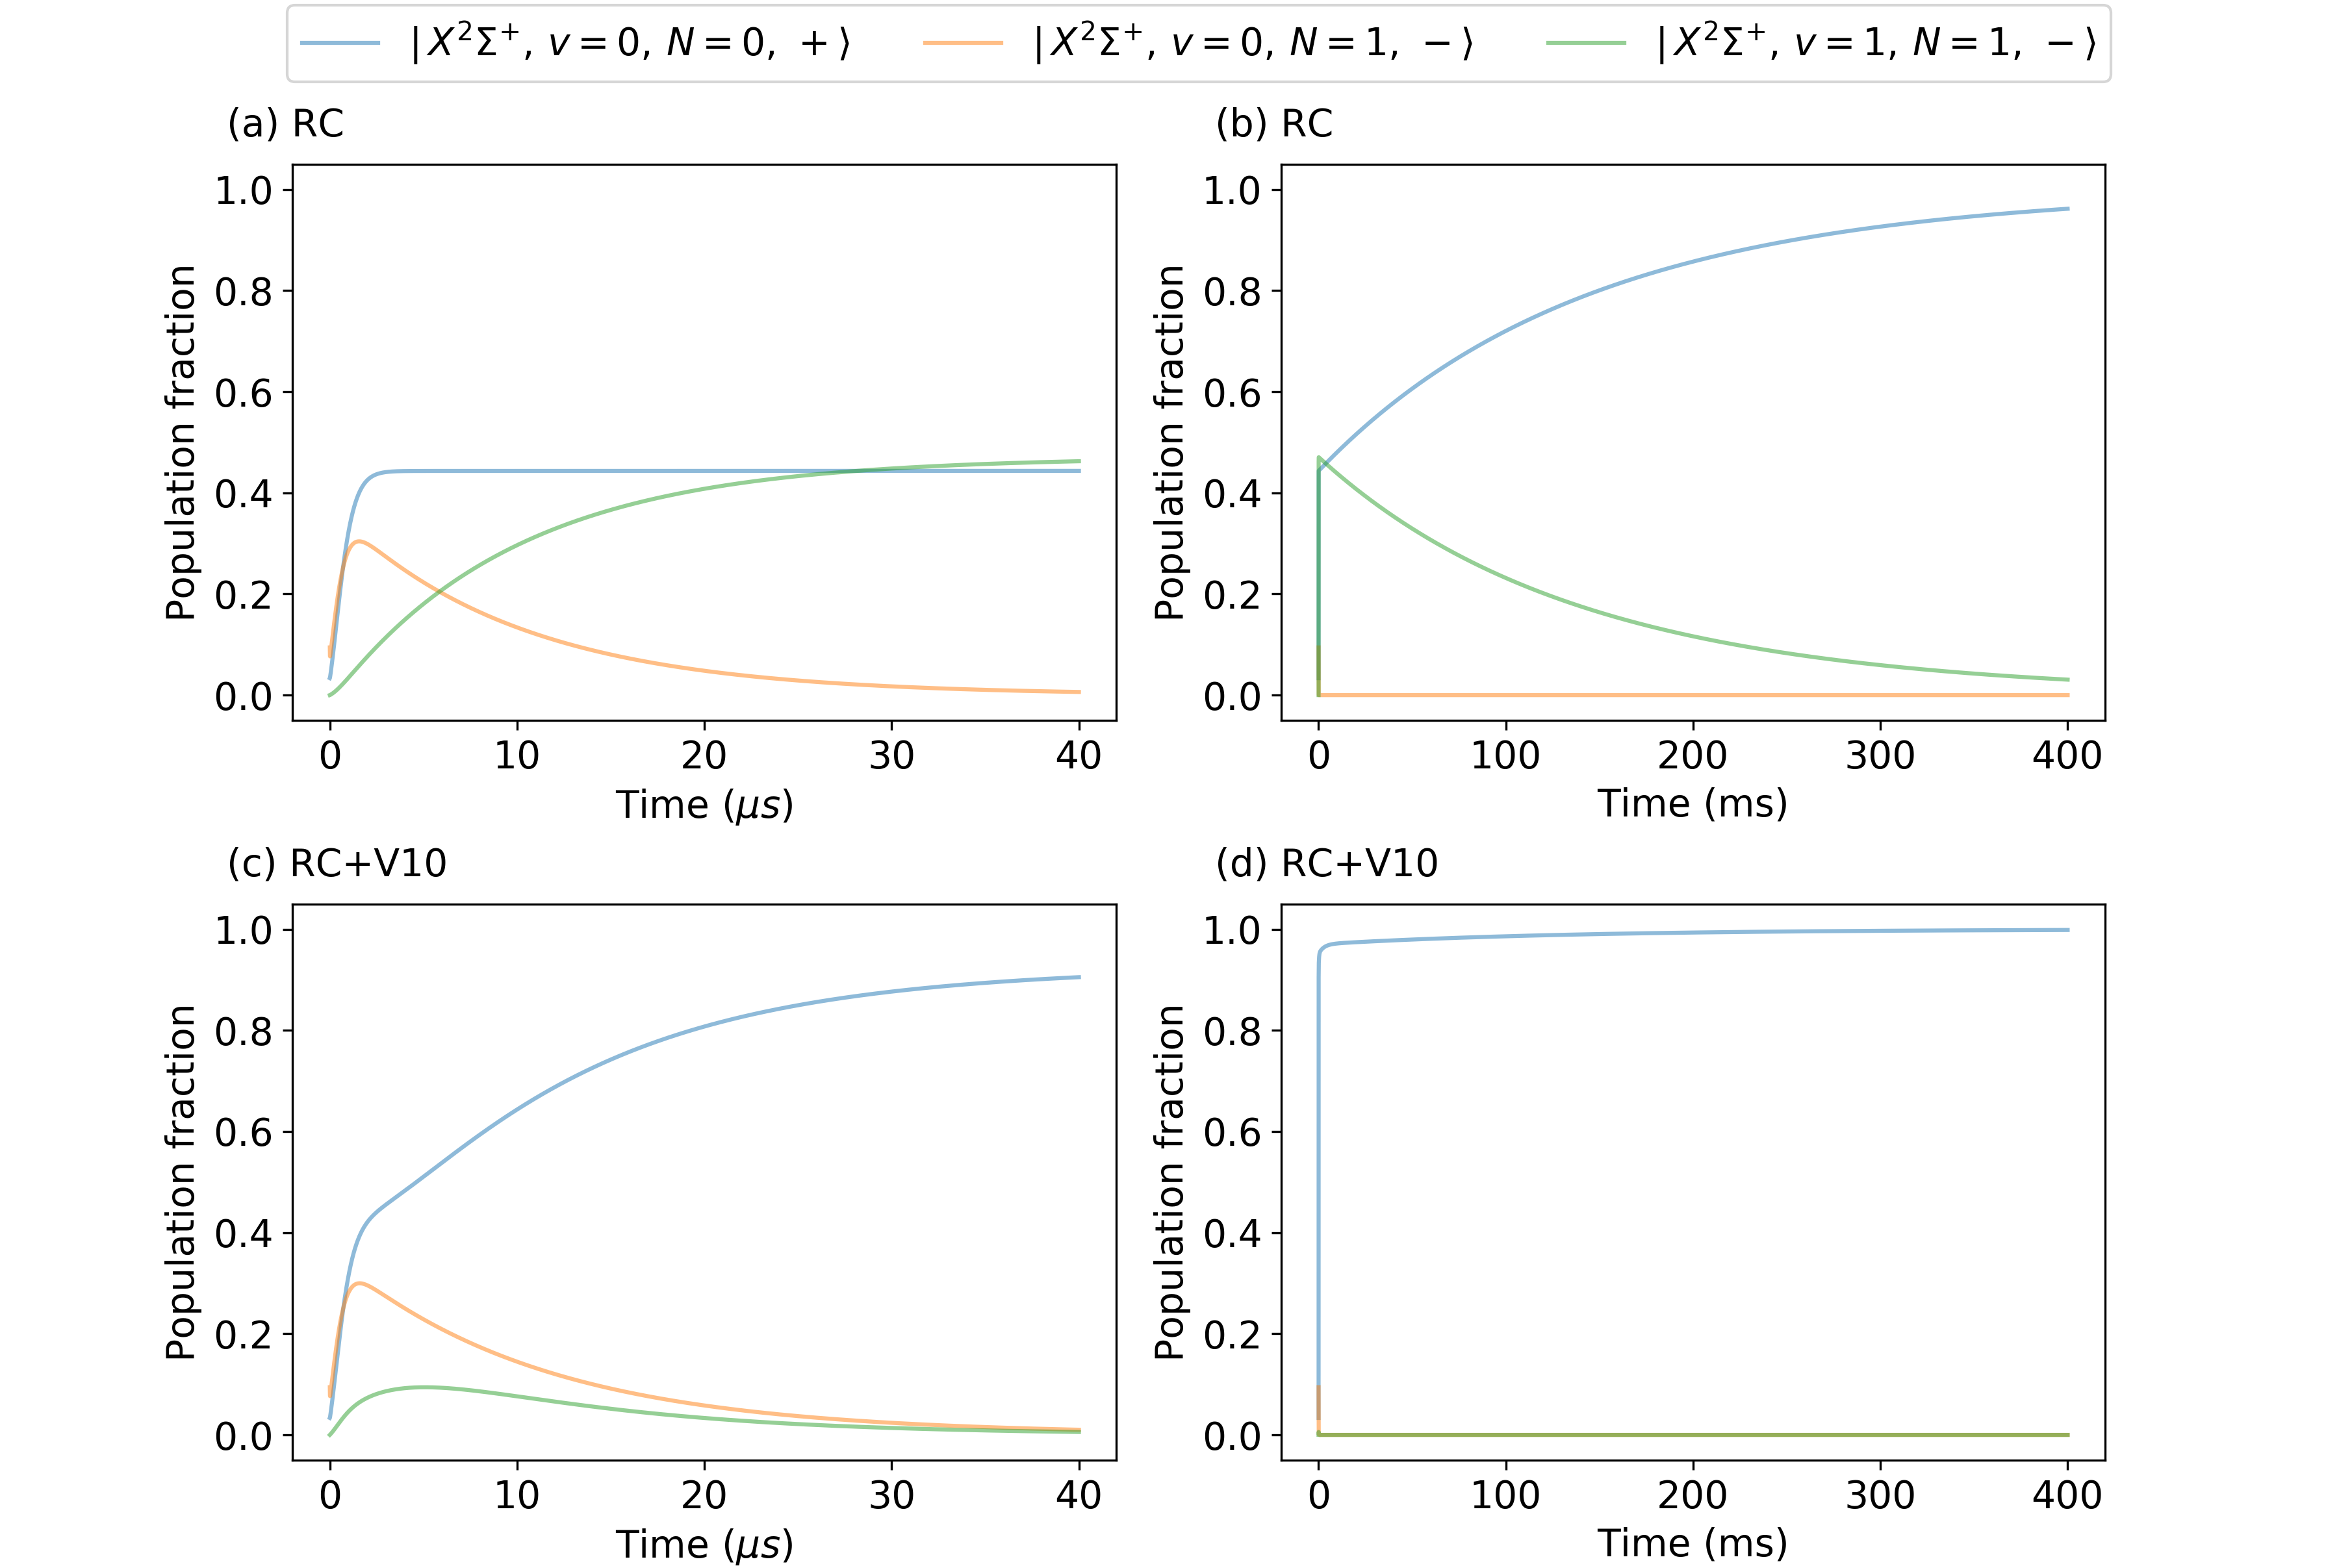
\includegraphics[width=12cm]{RC_RCv10} 
  \caption
  {The simulated population dynamics for rotational cooling: The top two plots are for the case with only applying the linearly polarized rotational cooling PFL (RC) for (a) 40 {\micro}s cooling time, and (b) 400 ms cooling time. The bottom two plots display the effect of applying the laser, v10 , which couples the transition between $\lvert X^2\Sigma^+, v''=1, N''=1, -\rangle$ and $\lvert X^2\Sigma^+, v''=0, N''=2, +\rangle$ in addition to the linearly polarized rotational cooling PFL for (c) 40 {\micro}s cooling time,and (d) 400 ms cooling time.
  }\label{RC_RCv10} 
\end{figure*}  

\begin{table}
\renewcommand{\arraystretch}{1.25}
\caption{The time it takes for the population at the rotational ground states to reach 63.2 $\%$ and 95.4 $\%$.}
\begin{tabular}{|c|c|c|}
%\hline
%\multicolumn{3}{|c|}{WTmetaD parameters} \\
\hline
Cooling condition & 63.2 $\%$ &  95.4 $\%$   \\ \hline
RC, HC & 276.2 ms & 1058 ms \\ \hline
RC and v10 & 80.0 {\micro}s & 2.0 ms \\ \hline
\end{tabular}
\label{RCHC_RCHCv10table}
\end{table}

\begin{figure*}[htbp!]
  \centering
  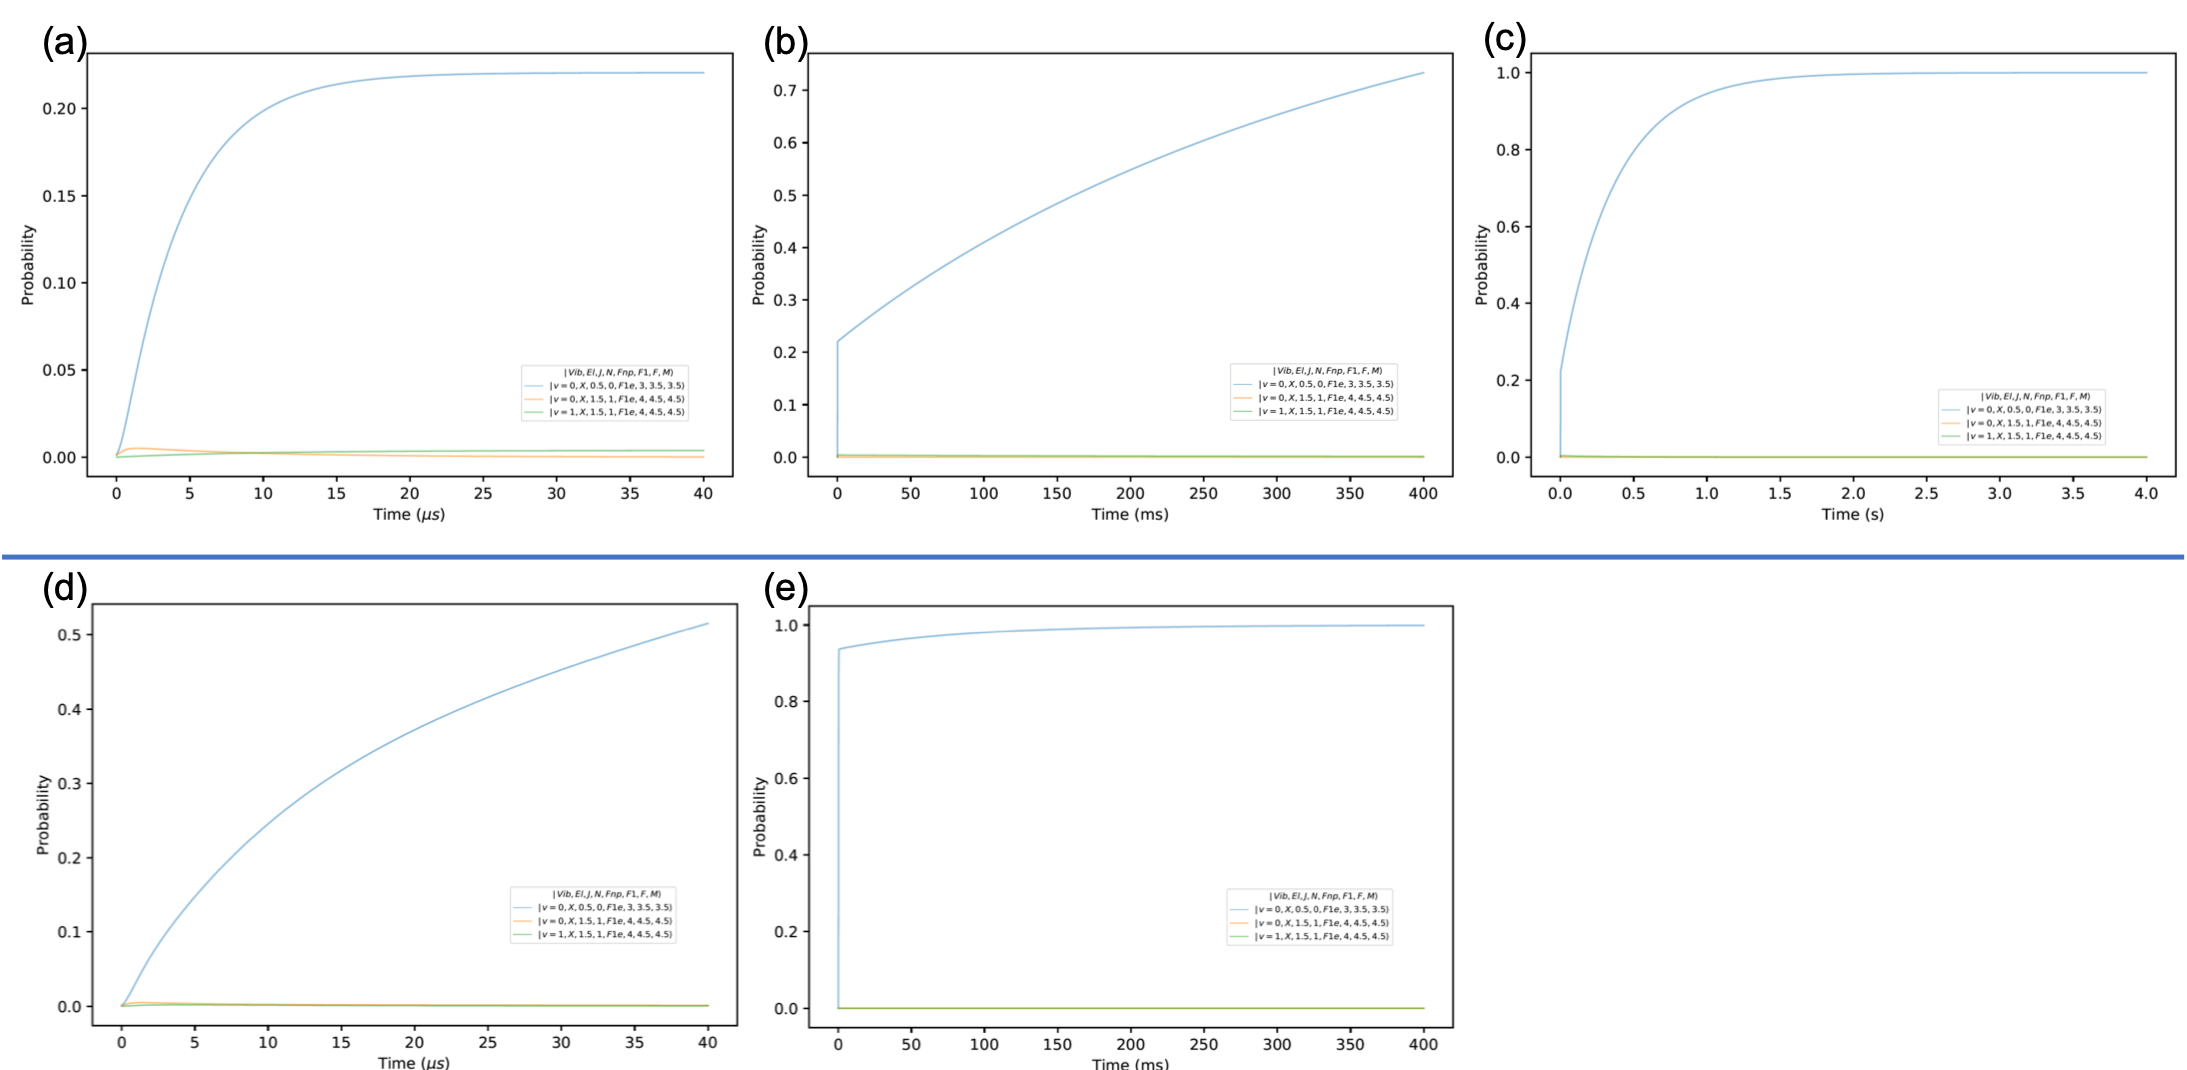
\includegraphics[width=18cm]{RCHC_RCHCv10}
  \caption
  { The simulated population dynamics for the single hyperfine state proparation: The top three plots are for the case with the linearly polarized rotational cooling PFL (RC) and the $\sigma^+$-polarized hyperfine cooling PFL for (a) 40 {\micro}s cooling time, (b) 400 ms cooling time and (c) 4 s cooling time. The bottom two plots display the effect of applying the laser, v10 , which couples the transition between $\lvert X^2\Sigma^+, v''=1, N''=1, -\rangle$ and $\lvert X^2\Sigma^+, v''=0, N''=2, +\rangle$ in addition to the linearly polarized rotational cooling PFL and the $\sigma^+$-polarized hyperfine cooling PFL for (d) 40 {\micro}s cooling time,and (e) 400 ms cooling time.
}\label{RCHC_RCHCv10}
\end{figure*}


In the case of adding a laser (v10) that couples the transition between the $\lvert X^2\Sigma^+, v''=1, N''=1, -\rangle$ and $\lvert X^2\Sigma^+, v''=0, N''=2, +\rangle$ states. The laser is set to have the bandwidth $\sim 15\, cm^{-1}$ centered at the wavelength $\sim$ 6.8 {\micro}m which should be able to achieved using a broadband Fabry-Perot quantum cascade laser. 

\section{Result and discussion}
From Fig. \ref{RC_RCv10} and Table \ref{RC_RC_v10table}, we compare the rotational cooling rate in two situations that we apply the linearly-polarized rotational cooling laser, RC, with/without adding the rovibrational coupling laser, v10, which couples the transition between $\lvert X^2\Sigma^+, v''=1, N''=1, -\rangle$ and $\lvert X^2\Sigma^+, v''=0, N''=2, +\rangle$ states.  By adding the v10 laser, the time it takes for the population in the rovibrational ground state, p$_0$, to reach 63.2 $\%$ is shorten from 49.5 ms to 9.4 {\micro}s. The time it takes for p$_0$ to reach 95.4 $\%$ also becomes faster from 307.4 ms to 49.5 ms.

In Fig. \ref{RCHC_RCHCv10}, we also show our simulation results in two situations which we apply the rotational cooling laser, RC, and the $\sigma^+$-hyperfine pumping laser, HC, with/without adding the rovibrational coupling laser, v10. In the case without the v10 laser applied, it can be seen that in the first tens of microsecond the population in the stretched hyperfine state increases to about $20\,\%$. Then after a second, the population will reach more than 90 $\%$, which has exceeded the theoretically achievable population of $65\,\%$ reported in the previous work using HD$^+$[cite]. The time scale to reach this amount of population is also much shorter which is the shortest time scale in the quantum state preparation for molecular ion that has ever been proposed. From Table \ref{RCHC_RCHCv10table}, we can also see that in the case with the v10 laser applied, the time it takes for the population in the stretched state of rovibrational ground state, p$_{0s}$, to reach 63.2 $\%$ is shorten from 276.2 ms to 80.0 {\micro}s. The time it takes for p$_{0s}$ to reach 95.4 $\%$ also becomes faster from 1058 ms to 2.0 ms.


\begin{table}
\renewcommand{\arraystretch}{1.25}
\caption{The time it takes for the population at the rotational ground states to reach 63.2 $\%$ and 95.4 $\%$.}
\begin{tabular}{|c|c|c|}
%\hline
%\multicolumn{3}{|c|}{WTmetaD parameters} \\
\hline
Cooling condition & 63.2 $\%$ &  95.4 $\%$   \\ \hline
RC & 49.5 ms & 307.4 ms \\ \hline
RC and v10 & 9.4 {\micro}s & 640.0 {\micro}s \\ \hline
\end{tabular}
\label{RC_RC_v10table}
\end{table}


\section{Conclusion}
In summary, we have proposed an enhanced method based on our previous experimental and computational result which is able to prepare the single molecular quantum state in an efficient way. 

\bibliographystyle{ieeetr}
\bibliography{../AlH+_references.bib}

	\end{document}  

